\documentclass[10pt,a4paper]{article}
\usepackage[latin1]{inputenc}
\usepackage{amsmath}
\usepackage{amsfonts}
\usepackage{amssymb}
\usepackage{graphicx}
\usepackage{subcaption}
\usepackage[left=2cm,right=2cm,top=2cm,bottom=2cm]{geometry}
\author{Steve Hughey}
\title{PHY 905 Project 2: Molecular dynamics simulation of argon gas}
\begin{document}
\maketitle
\section{Overview}
The object of this project was to write and demonstrate a code for simulating the molecular dynamics of a lattice of Argon atoms using the Verlet integration algorithm. Section 2 reviews both the algorithm and the physical theory upon which the model is based, and implementation details are outlined. Section 3 presents results from the code. Section 4 summarizes and evaluates the success of the project.
\section{Theory \& Implementation}
\subsection{Background}
Molecular dynamics methods help solve a class of problems involving a system of interacting particles, each subject to Newton's second law of motion $\mathbf{F}=m\mathbf{a}=mD_t^2\mathbf{x}$, where $\mathbf{F}$ is the force acting on a particle, $m$ is the particle's mass, $\mathbf{x}$ is the position of the particle in space, $\mathbf{a}$ is the particle's acceleration, and $D_t$ denotes the time derivative operator. In this report, we will consider the problem of an argon gas lattice, where the pair interaction potential between two particles a distance $R>0$ away from each other is known as the Lennard-Jones potential and is given by

\begin{align}
 V(R) = 4\varepsilon \left( \left(\frac{\sigma}{R}\right)^{12} - \left(\frac{\sigma}{R}\right)^{6} \right),
\end{align}

where $\varepsilon$ is the magnitude of the minimum value of the potential, and $\sigma$ is the distance at which the potential becomes null. The two terms in the expression represent both a short-range repulsion interaction to account for the repulsive electric force when the electron clouds of two atoms approach each other (Pauli repulsion), and a long-range attractive force famously known as the van der Waals force. The force due to this potential is given by $\mathbf{F}=D_r V(r) \hat{R}$. Assuming no external forces in the lattice, we can set $D_rV(r)\hat{R}=m D_t^2 \mathbf{x}$, giving a differential equation in time for the position $\mathbf{x}$ of the particle. Typically, the differential equation is solved by means of the Verlet integrator, which is described in the next section. For purposes of simplicity in this report, we work in normalized units and thus set $\varepsilon = \sigma = 1$.

\subsection{Velocity Verlet algorithm}
Consider a collection of particles in space, each with mass $m_i=1$. For each particle, we can write Newton's second law as

\begin{align}
\mathbf{F}_i(\mathbf{x}_i,t)=m_iD_t^2\mathbf{x}_i(t),
\end{align}

where $\mathbf{F}_i$ denotes the force from the Lennard-Jones potential interactions with all other atoms in the system. In order to solve this differential equation numerically, we use an integrator known as the velocity Verlet algorithm. This approach involves using relationships between position, velocity, acceleration, and force to develop an explicit finite differencing scheme. Finite differencing schemes rely on the fact that a function $f$ at the point $(t+\Delta t)$ can be written in terms of $f(t)$ and its derivatives via the Taylor expansion:

\begin{align}
f(t+\Delta t) = f(t) + (\Delta t) D_t f(t) + \frac{1}{2}(\Delta t)^2 D_t^2 f(t) + \mathcal{O}((\Delta t)^3).
\end{align}

For well-behaved functions, when $\Delta t < 1$ is small, i.e. the point $t+\delta t$ is very close to $t$, each successive term in the expansion becomes exponentially smaller than the previous term. For small enough step sizes $\Delta t$ we can omit the cubic term and all those that follow. Let the function $f$ be the position in space $\mathbf{x}_i$ of the $i^{th}$ atom. We know that the velocity is related to the position by $\mathbf{v}_i=D_t \mathbf{x}_i$, and that the acceleration is related to the position by $\mathbf{a}_i=D_t^2\mathbf{x}_i$, We can then obtain an expression for the position $\mathbf{x}_i$ of the $i^{th}$ particle:

\begin{align}
 \mathbf{x}_i(t+\Delta t) = \mathbf{x}_i(t) + \mathbf{v}_i(t)\Delta_t + 0.5\mathbf{a}_i(t)(\Delta t)^2
\end{align}

The velocity Verlet algorithm is a four-step iteration that exploits this relationship to solve for the position of each particle at every time step. For each particle $i$, the algorithm comprises the following four steps:

\begin{enumerate}
 \item Partially update the velocity of each particle using the acceleration at the current time step:\\
  \begin{align}
   \mathbf{v}_i^{(n+1/2)} = \mathbf{v}_i^{(n)} + \frac{\Delta t}{2} \mathbf{a}_i^{(n)}. \label{eq:alg_beg}
  \end{align}
  Here, superscripts denote time steps, i.e. $\mathbf{x}_i^{(n)}=\mathbf{x}_i(n\Delta t)$
  \item Using the partially-updated velocity, update the position of each particle:\\
  \begin{align}
   \mathbf{x}_i^{(n+1)} = \mathbf{x}_i^{(n)} + (\Delta t) \mathbf{v}_i^{(n+1/2)}
  \end{align}
  \item Compute the pair potential force $\mathbf{F}$ at the next time step for each pairwise interaction and use it to update the acceleration:\\
  \begin{align}
   \mathbf{a}_i^{(n+1)} = \sum_{j \neq i} \hat{r}_{ij} D_r V(r)|_{r=r_{ij}}
  \end{align}
  All masses in this system are normalized to a value of 1, so in this instance the force is equal to the acceleration.
  \item Complete the update of the velocity of each particle using the new value of the acceleration:
  \begin{align}
   \mathbf{v}_i^{(n+1)} = \mathbf{v}_i^{(n+1/2)} + \frac{\Delta t}{2} \mathbf{a}_i^{(n+1)}.\label{eq:alg_end}
  \end{align}
\end{enumerate}

\subsection{Implementation}
In the case considered here, we initialize each particle with a position in an fcc lattice (see Fig. \ref{fig:Lattice}) and a random velocity whose cartesian components are generated using the Box-Muller distribution. The velocity mean over all particles is computed and removed from the initial value of each particle's velocity such that the ensemble has zero mean velocity to start. Accelerations are initialized to zero, and a target temperature is chosen. At each time step, Eq. \ref{eq:alg_beg}-\ref{eq:alg_end} are solved in sequence. In order to guide the system toward the target temperature, the velocities of each particle are rescaled periodically in accordance with the following temperature-kinetic energy relationship (Maxwell-Boltzmann):

\begin{align}
3(N_{atoms}-1)k_B T = \sum_i m_i |\mathbf{v}_i|^2
\label{eq:kine}
\end{align}

After some number of rescalings, the temperature should reach the target and remain relatively close for the remainder of the simulation. In addition to these considerations, it is also important that we recognize the spatial periodicity of the structure we are modeling. If a particle leaves the lattice stage right at some time step, we must ensure that it re-enters the lattice stage left at the following time step. This constraint on the system is called a periodic boundary condition, and it can be imposed on the particle positions using simple modulo arithmetic: if any cartesian component of the position becomes negative or larger than the portion of the lattice under consideration, the dimension of the lattice among that direction is subtracted repeatedly from that quantity until it lies inside the domain once again. With the periodicity of the system in mind, we must also ensure that the Lennard-Jones potential for any pair $(i,j)$ of particles is computed with the shortest distance between the two particles in the domain or their images in neighboring domains.

\section{Results}
 \subsection{Validation Example}
  \begin{figure}[ht!]
  \centering
  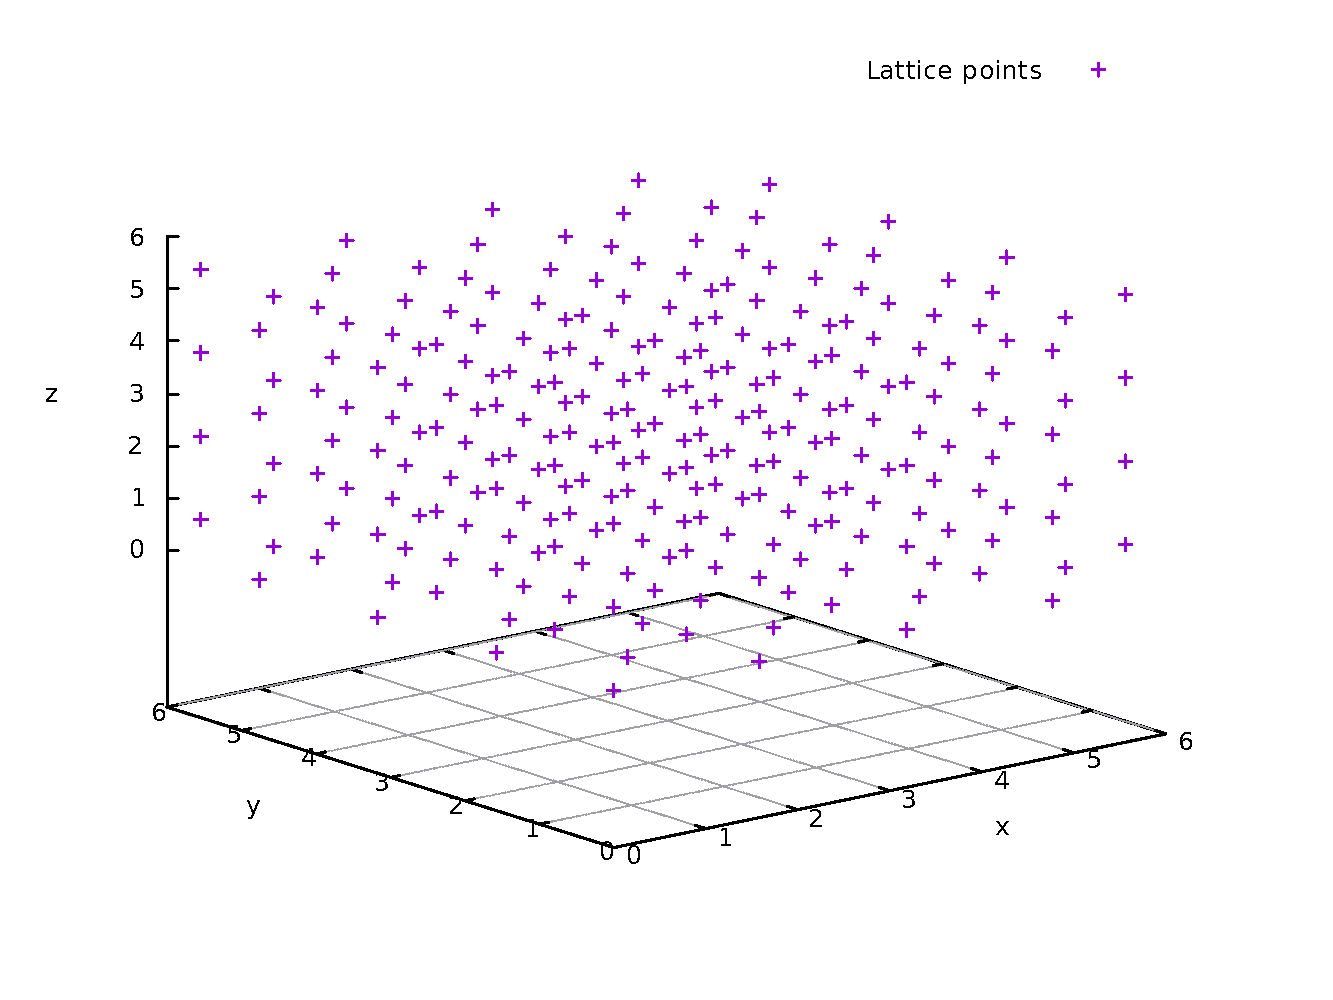
\includegraphics[width=0.6\linewidth]{figs/lattice.pdf}
  \caption{Atom distribution in the fcc lattice described in this section}
  \label{fig:Lattice}
 \end{figure}
 In this section, we demonstrate the implementation discussed in the previous section by means of a validation example. The face-centered cubic (fcc) lattice in this section is chosen to be $4 \times 4 \times 4$ for a total of 64 cells and 256 total atoms, and can be seen in Fig. \ref{fig:Lattice}. Setting the target temperature $T=2$ and the time step $\Delta t = 0.004$ units of $2.17 ps$, the simulation was run for 5000 time steps. Fig. \ref{fig:Evst} shows the energy of the lattice versus time for the stated configuration. In order to converge upon the target temperature, the particle velocities were chosen to be rescaled every 20 time steps until the 500th time step, occurring in Fig. \ref{fig:Evst} just before $t=2$. The temperature is shown in Fig. \ref{fig:Tempvst}. From these figures, the effect of the rescaling is clear: the temperature quickly approaches the target temperature before settling into a state of fluctuation about the target, while the energy of the system approaches a stationary value similarly quickly, fluctuates some, and ceases fluctuating when velocity rescaling is discontinued. This demonstrates that the energy of the system is conserved. Fig. \ref{fig:Tracer} shows the time evolution of the trajectory of a tracer particle in the lattice.
 \begin{figure}
  \centering
  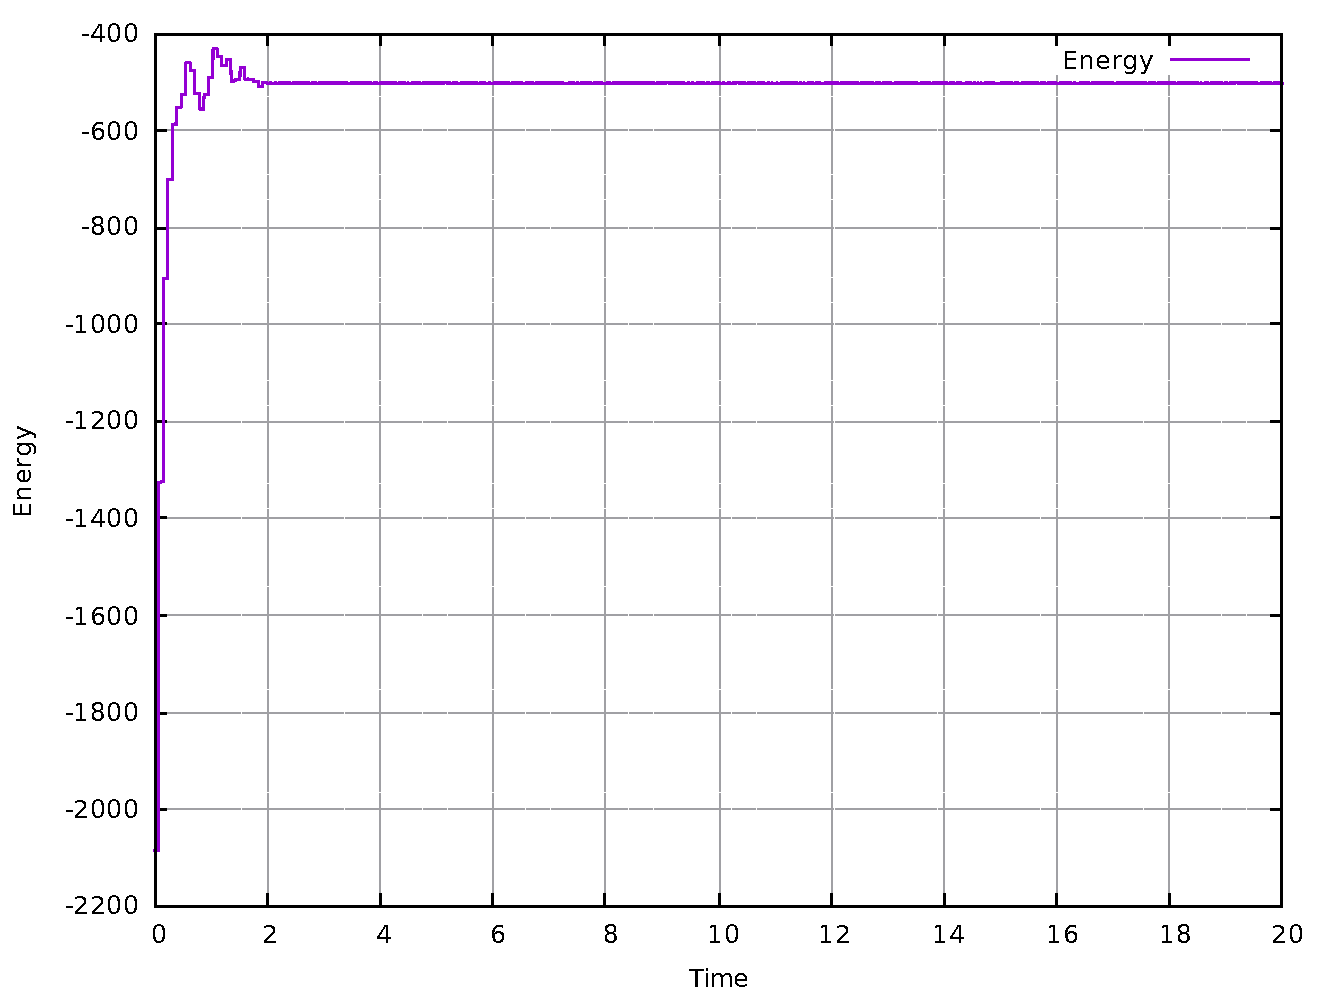
\includegraphics[width=0.6\linewidth]{figs/energyVsTime.pdf}
  \caption{Energy of the lattice vs. time}
  \label{fig:Evst}
 \end{figure}
 
 \begin{figure}
  \centering
  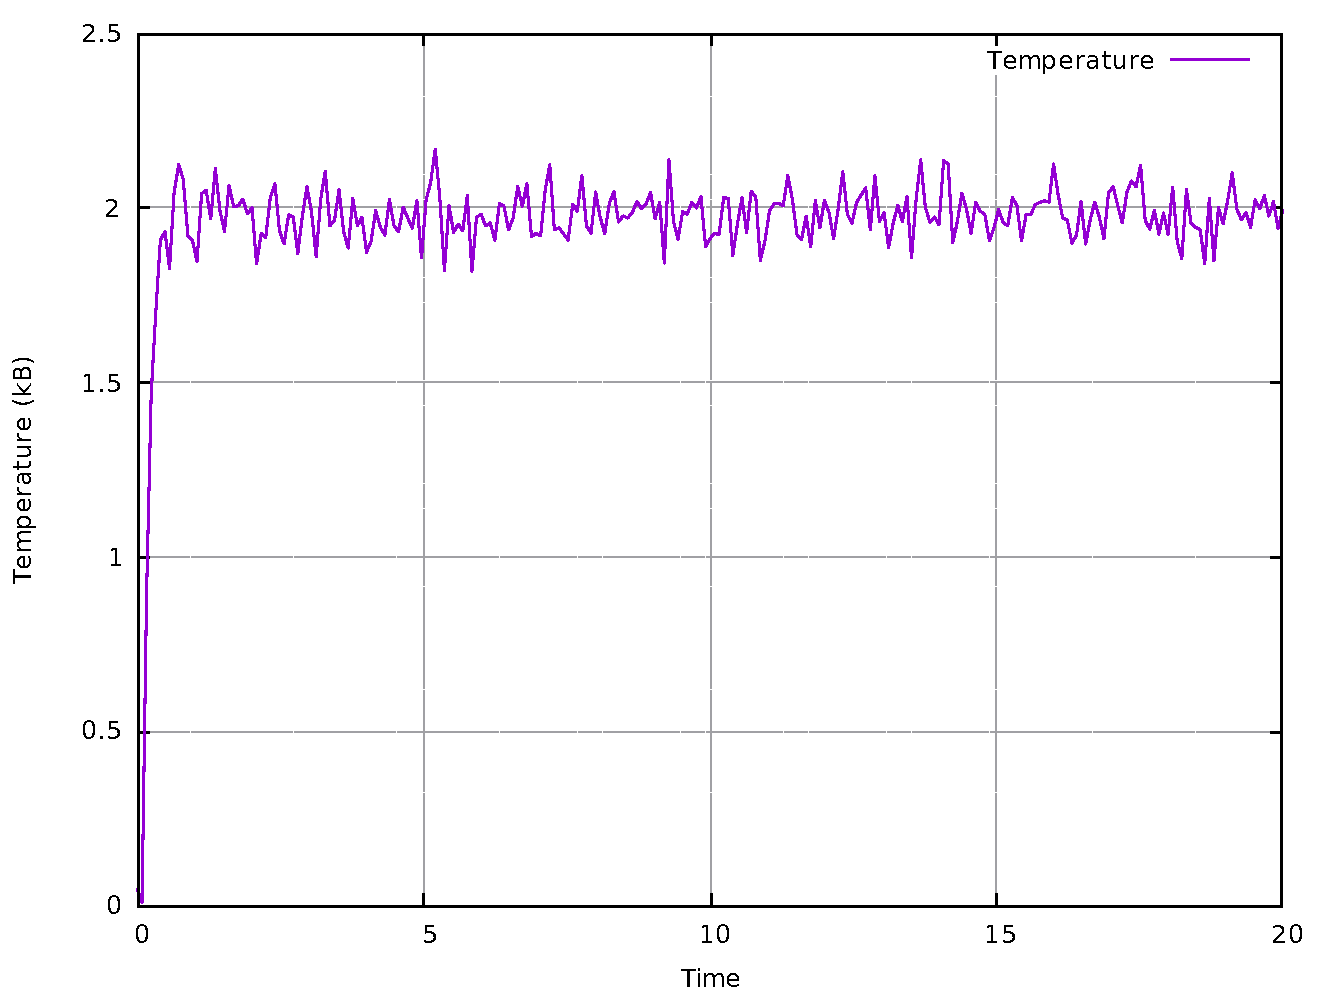
\includegraphics[width=0.6\linewidth]{figs/tempVsTime.pdf}
  \caption{Temperature of the lattice vs. time}
  \label{fig:Tempvst}
 \end{figure}
 
 \begin{figure}[ht!]
  \centering
  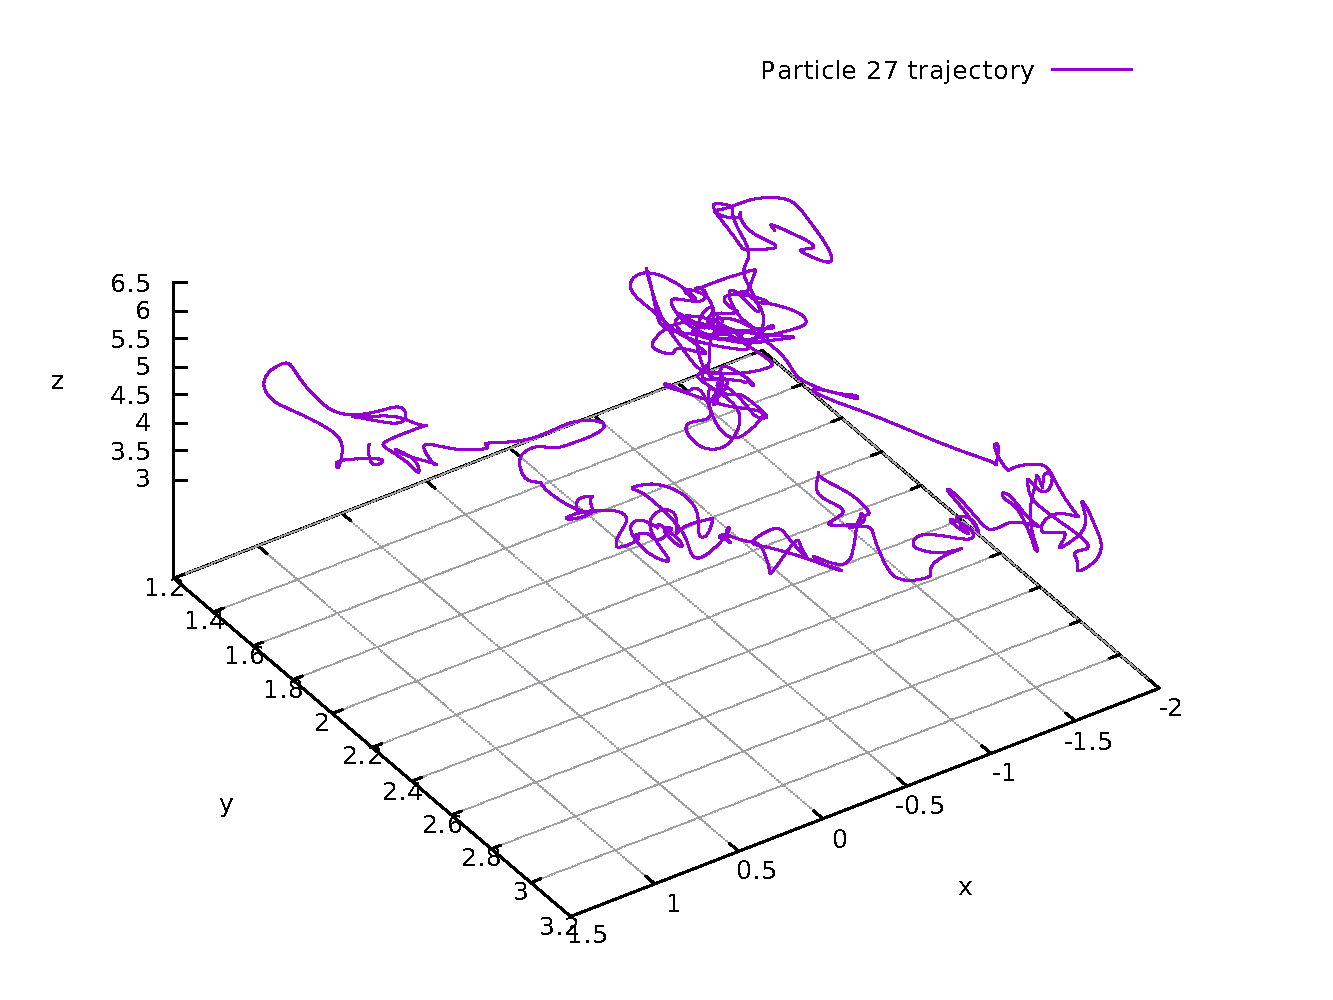
\includegraphics[width=0.6\linewidth]{figs/particlePath.pdf}
  \caption{Trajectory of a tracer particle in the lattice vs. time}
  \label{fig:Tracer}
 \end{figure}
 
 \subsection{Other Results}
 In this section we consider a 2$\times$2 lattice with 32 total atoms, run for 1000 time steps. Fig. \ref{fig:Evstemp} shows the energy of this system as the temperature is increased by $\Delta T=0.01$ units of $k_B$ from $T=1$ to $T=6$. As the temperature increases, the energy in the system increases accordingly. This reflects the earlier relationship \eqref{eq:kine} used in the velocity rescaling process. The kinetic energy in the system is linearly proportional to the temperature.
 
 \begin{figure}[ht!]
  \centering
  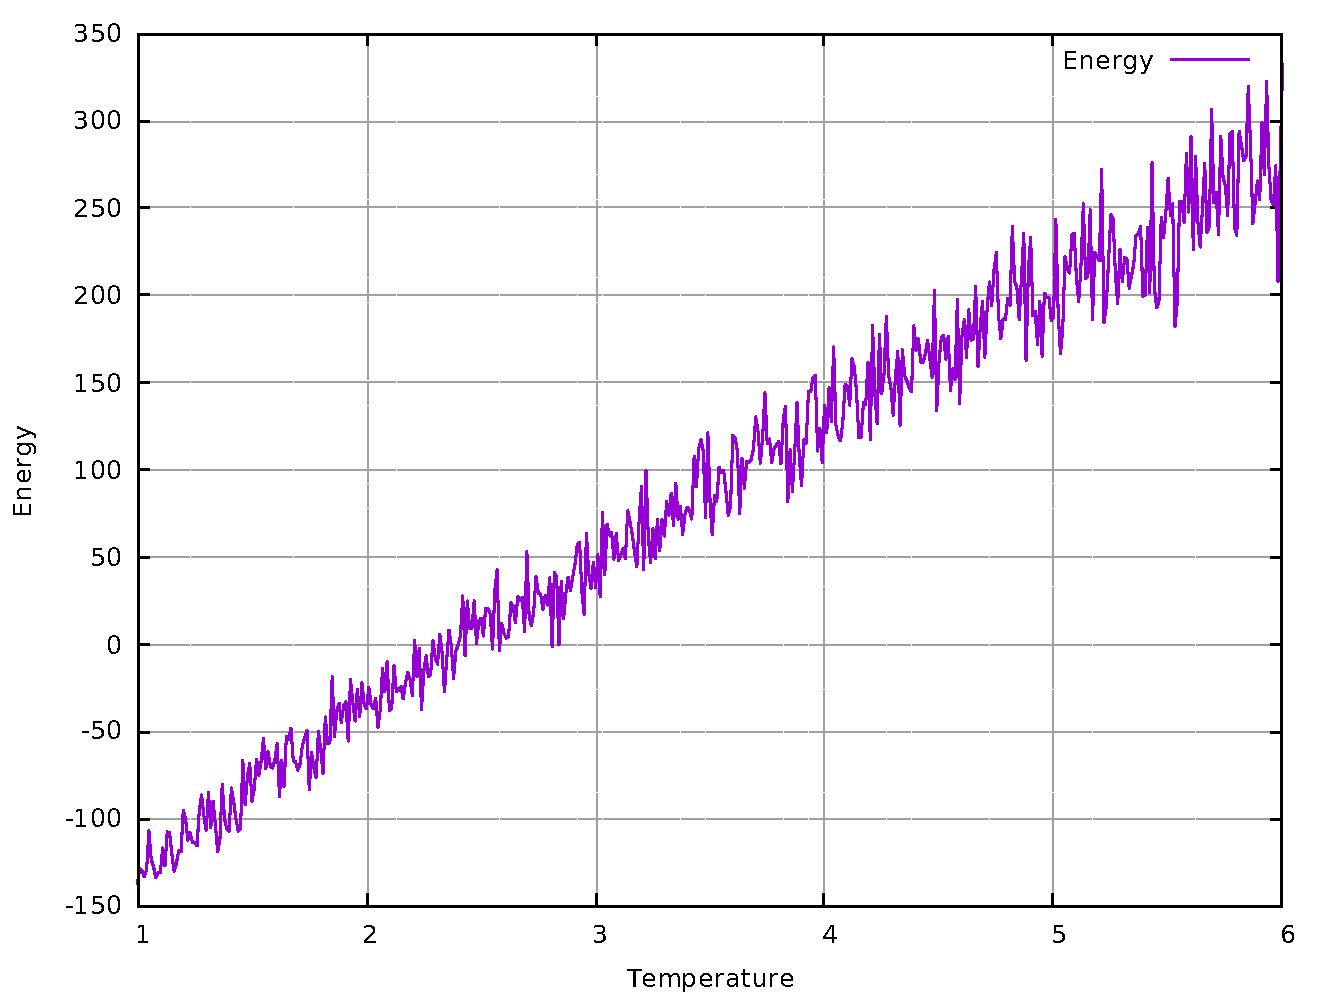
\includegraphics[width=0.6\linewidth]{figs/energyVsTemp.pdf}
  \caption{Energy of the lattice vs. temperature}
  \label{fig:Evstemp}
 \end{figure}

 \begin{figure}[ht!]
 \centering
 \begin{subfigure}[b]{0.3\linewidth}
  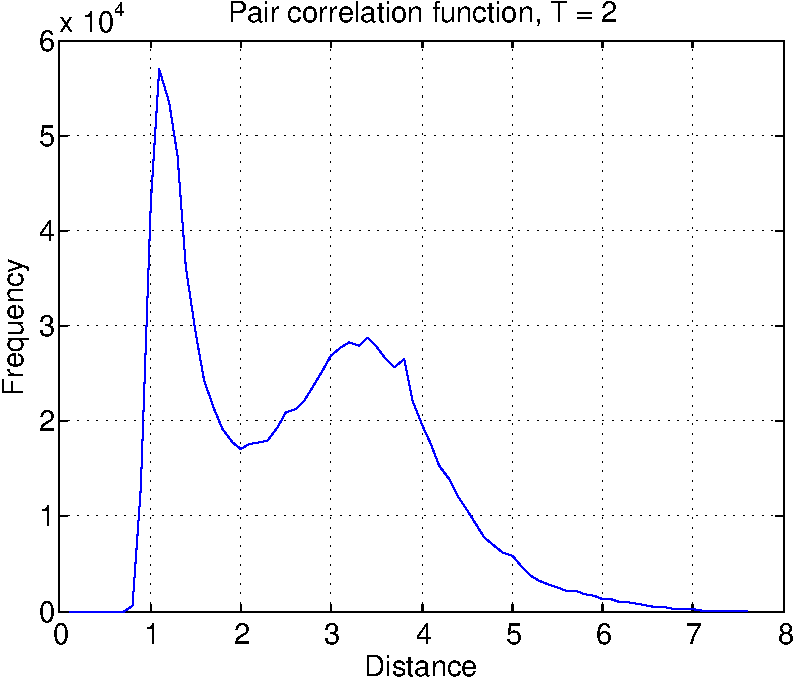
\includegraphics[width=\textwidth]{figs/pair_corr_Teq2-crop.pdf}
  \caption{$T=2$}
  \label{fig:pcorr2}
 \end{subfigure}
 \begin{subfigure}[b]{0.3\linewidth}
  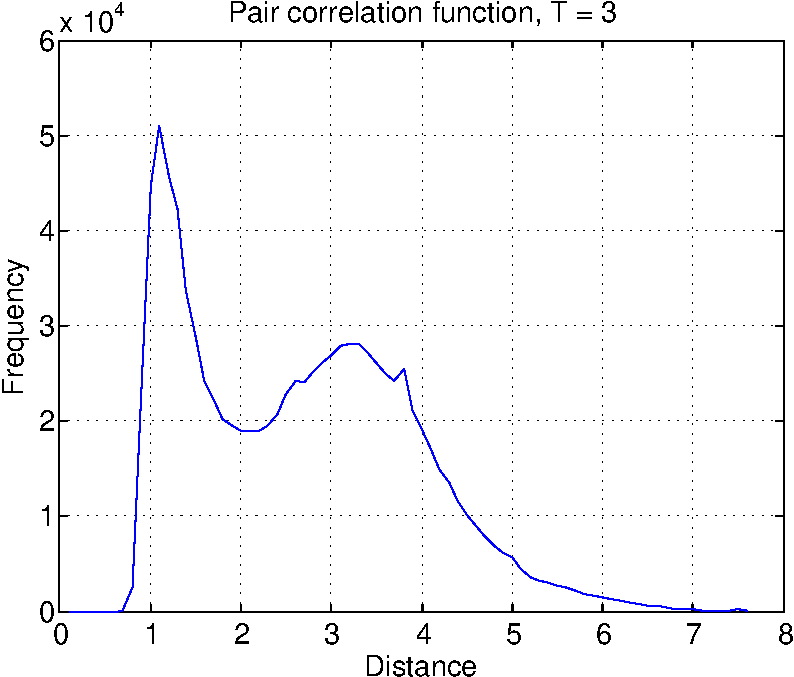
\includegraphics[width=\textwidth]{figs/pair_corr_Teq3-crop.pdf}
  \caption{$T=3$}
  \label{fig:pcorr3}
 \end{subfigure}
 \begin{subfigure}[b]{0.3\linewidth}
  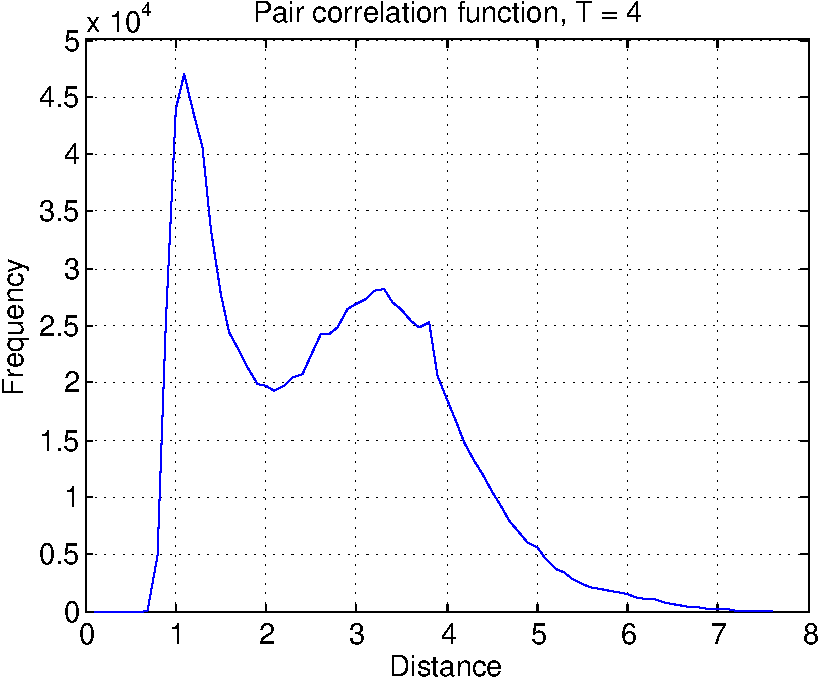
\includegraphics[width=\textwidth]{figs/pair_corr_Teq4-crop.pdf}
  \caption{$T=4$}
  \label{fig:pcorr4}
 \end{subfigure}
 
  \begin{subfigure}[b]{0.3\linewidth}
  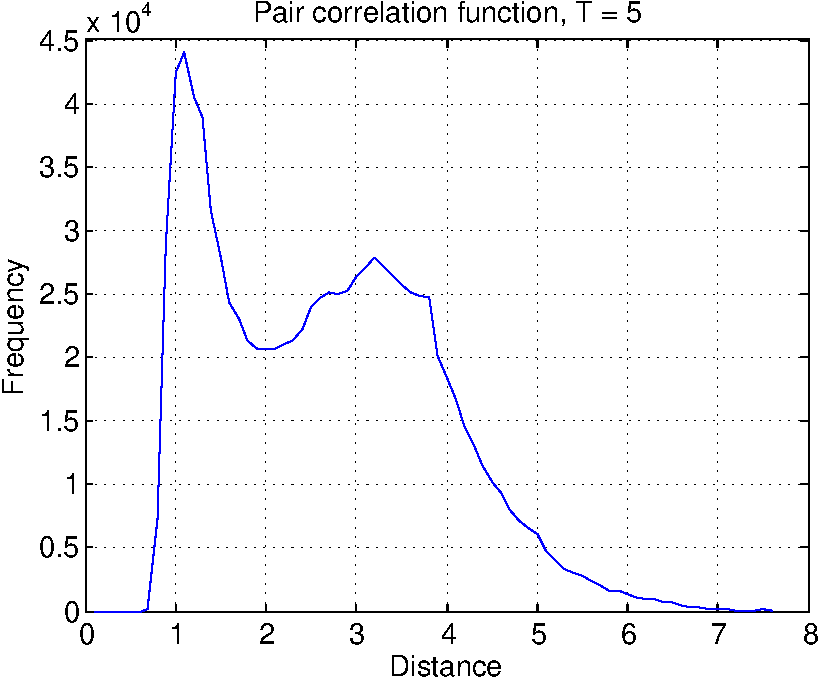
\includegraphics[width=\textwidth]{figs/pair_corr_Teq5-crop.pdf}
  \caption{$T=5$}
  \label{fig:pcorr5}
 \end{subfigure}
 \begin{subfigure}[b]{0.3\linewidth}
  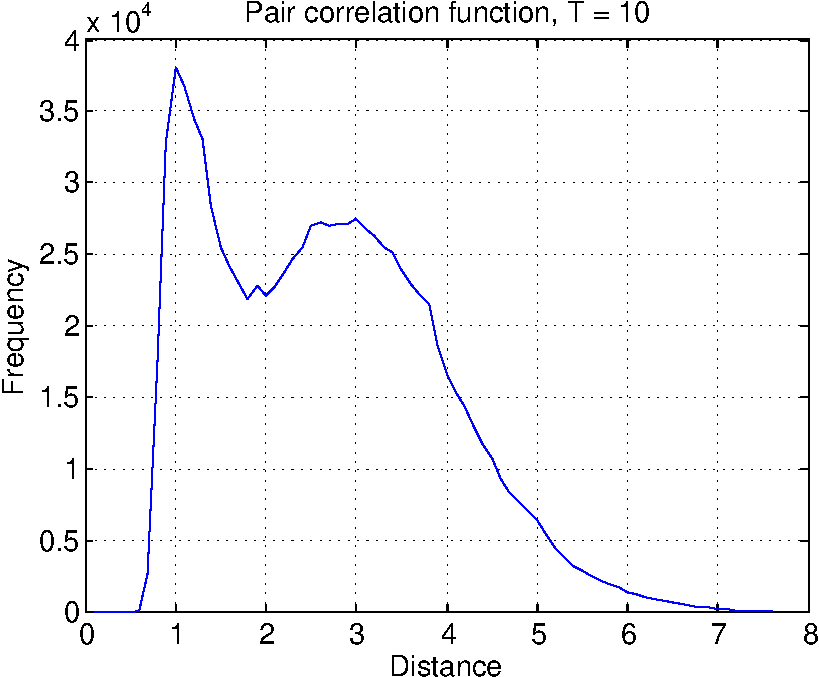
\includegraphics[width=\textwidth]{figs/pair_corr_Teq10-crop.pdf}
  \caption{$T=10$}
  \label{fig:pcorr10}
 \end{subfigure}
 \begin{subfigure}[b]{0.3\linewidth}
  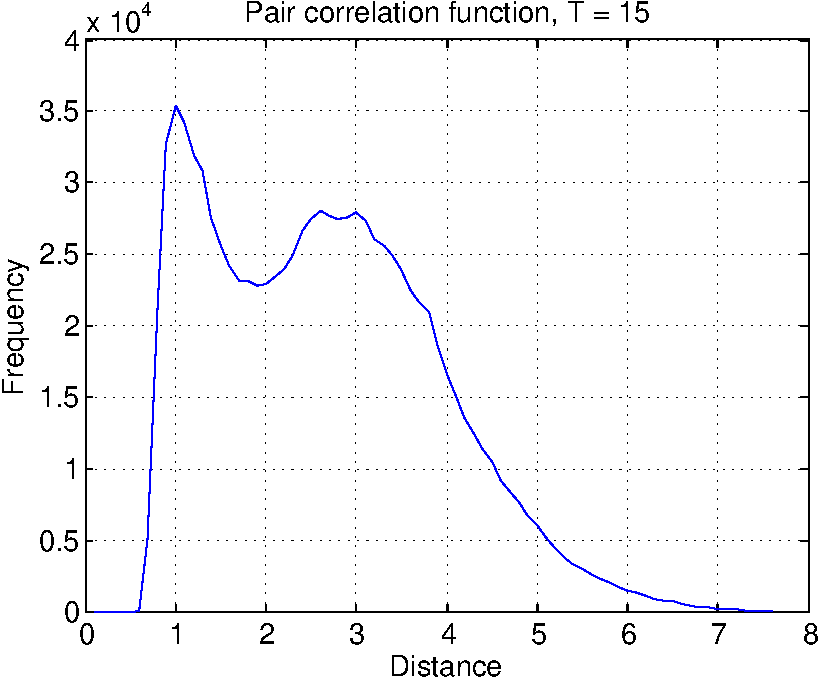
\includegraphics[width=\textwidth]{figs/pair_corr_Teq15-crop.pdf}
  \caption{$T=15$}
  \label{fig:pcorr15}
 \end{subfigure}
 
 \caption{Pair correlation functions for a range of temperatures.}
 \label{fig:pcorrs}
\end{figure}

Fig. \ref{fig:pcorrs} shows the pair correlation function of the ensemble for a range of temperatures. The pair correlation function is effectively the probability distribution of the distance between any pair of particles. This was computed by calculating all the particle pair distances at each time step of the simulation and sorting the magnitudes into bins of size $dr=0.1$. For all temperatures chosen, the pair correlation function has a distinct shape that can be attributed to the terms of the Lennard-Jones interaction force. The short-range repulsive interaction $\sim r^{-12}$ keeps individual atoms from coming too close to each other, and this is evinced by the short-distance behavior of the pair correlation functions at all temperatures. The peak value of the function occurs around $r=1$ for lower temperatures, but as the temperature increases, the spread of this region of the function increases because the increase in thermal energy in the system leads to an increase in pressure for a fixed volume. This additional energy counteracts the repulsive force. The peak distance remains fixed at $r=1$ because we chose the potential to be zero at that point. The attractive Lennard-Jones force $\sim -r^{-6}$ accounts for the secondary peak starting at $r\approx3.3$ for $T=2$ and shifting down to $r\approx 2.6$ for $T=15$. The potential in this region is purely attractive. The frequency of this peak remains relatively unchanged throughout the range of temperatures, decreasing only slightly as the temperature increases.
 
\section{Conclusion}
In this report, we have summarized the velocity Verlet algorithm for molecular dynamics simulations and discussed implementation details. We have also shown results for a Fortran 90 implementation of this algorithm, and the computed quantities agreed with the expected behavior of the system. The Fortran code used to produce the results is available on the ICCP class page on GitHub.
\end{document}